% !TEX root = document.tex

\chapter{\label{chap:webdsl}WebDSL}

  In this chapter we describe WebDSL. WebDSL is a domain-specific language for developing web applications. The language incorporates ideas from various web programming frameworks and produces code for all tiers in a web application \autocite{Groenewegen2020}. Ever since its introduction over 15 years ago \autocite{Visser2007}, WebDSL has been a vehicle for research (cite some papers here) and on top of that, it is the programming language underpinning several applications used daily by thousands of users. Examples of WebDSL applications include:

  \begin{itemize}
    \item \textbf{WebLab}: An online learning management system, used by the Delft University of Technology.
    \item \textbf{conf.researchr.org}: A domain-specific content management system for conferences, used by most ACM SIGPLAN and SIGSOFT conferences.
    \item \textbf{researchr.org}: A platform for finding, collecting, sharing, and reviewing scientific computer science related publications.
  \end{itemize}

  In WebDSL, all aspects of web programming are defined in the same language which creates an opportunity for strong static consistency checking \autocite{Hemel2011}. The data model is defined using entities, which are automatically translated to a database representation. These entities can be passed as arguments of pages without the need to explicitly fetch data from the database. Large amounts of boilerplate code are abstracted over by WebDSL, by providing built-in but customizable functionality for access control, relations between entities and data validation. This combination of features allows WebDSL developers to efficiently create functioning prototypes while providing the functionality to make it scale and customizable.

  The rest of this chapter showcases the different aspects of WebDSL and zooms in on its non-trivial features. First, in \cref{sec:ui} we will describe how WebDSL offers functionality for creating web user interfaces. Next, in \cref{sec:data-model} we illustrate how the language manages data models. Thirdly, \cref{sec:access-control} contains information about WebDSL's solution for access control and in \cref{sec:functions} we highlight interesting aspects of its general-purpose object-oriented function code. We conclude this chapter by elaborating on the current implementation of the WebDSL static analysis in \cref{sec:current-implementation}.

  \section{\label{sec:ui}User Interfaces}

    The user interface of an application is the part of the system that the user interacts with. Through the user interface, users are able to navigate the system and manipulate its data.

    \subsection{\label{subsec:building-blocks}Building Blocks: Pages, Templates and Template Elements}

      In a WebDSL application, the user interface is exposed to the user via pages that are accessible from the browser. In WebDSL, pages are defined by their unique name and can optionally take arguments that directly correspond with the path of the webpage.

      Templates are reusable definitions of user interface code that can be included on pages and can be nested in other templates. \Cref{fig:webdsl-pages-and-templates} shows an example of an application with two pages, the \texttt{root} page and the \texttt{recipe} page, with navigation between them and a reusable template called \texttt{linkToRecipe} that creates a link to the recipe page with an argument of type string. The recipe page also takes one argument of type string which is visible in the URL path.

      \begin{figure}
        \begin{subfigure}[t]{0.45\textwidth}
          \begin{minted}[firstline=1]{\webdsl}
application app
  page root {
    title { "Cookbook" }

    header { "Recipes" }

    linkToRecipe("Lasagne")
    linkToRecipe("Pancakes")
    linkToRecipe("Tomato Soup")
  }

  page recipe(s : String) {
    title { "Cookbook: ~s" }

    navigate root() {
      "Back to homepage"
    }

    header { "~s" }

    "Welcome to the recipe page for ~s!"
  }

  template linkToRecipe(s : String) {
    par {
      navigate recipe(s) {
        "View recipe for ~s"
      }
    }
  }
          \end{minted}
          \caption{\label{fig:webdsl-pages-and-templates-webdsl}WebDSL code}
        \end{subfigure}
        \begin{subfigure}[t]{0.55\textwidth}
          \begin{subfigure}[t]{1\textwidth}
            \capstart
            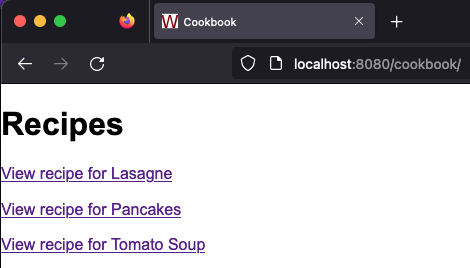
\includegraphics[width=\textwidth]{../img/webdsl-pages-templates-root}
            \caption{\label{fig:webdsl-pages-and-templates-root-page}Root page}
          \end{subfigure}
          \begin{subfigure}[t]{1\textwidth}
            \capstart
            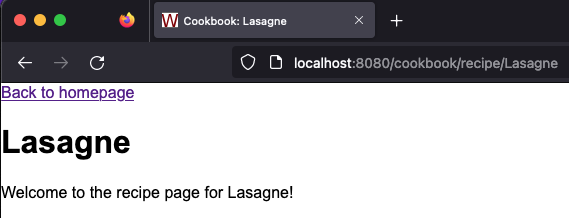
\includegraphics[width=\textwidth]{../img/webdsl-pages-templates-recipe}
            \caption{\label{fig:webdsl-pages-and-templates-recipe-page}Recipe page}
          \end{subfigure}
        \end{subfigure}
      \caption{\label{fig:webdsl-pages-and-templates}An example of a simple WebDSL application with two pages, navigation and reusable templates.}
      \end{figure}

      The \texttt{navigate} calls are references to other pages in the application. Because all pages are known at compile time, WebDSL ensures that all navigation within an application refers to existing pages, and that the passed types are correct. Referring to a non-existing page or passing the wrong argument types would show an error in the WebDSL development environment and while compiling the application.
      
      Other than pages and templates and navigation between pages, the application uses various calls to built-in template such as \texttt{title}, \texttt{header} and \texttt{par}. These built-in templates are translated to their respective HTML elements \texttt{<title></title>}, \texttt{<h1></h1>} and \texttt{<p></p>}. WebDSL also supports directly using HTML elements with their usual syntax such as \texttt{<div>"text"</div>}, but using template-style code such as \texttt{div \{ "text" \}} is the convention in WebDSL.

      Outputting text on a webpage in WebDSL can be done by typing the text between quotes in a template or page, as is shown in the example cookbook application of \cref{fig:webdsl-pages-and-templates}.

      Using the concepts described in this subsection, developers are able to create static websites with WebDSL. However, a powerful aspect of WebDSL is its ability to create dynamic pages without requiring much boilerplate code.

    \subsection{\label{subsec:request-processing}Request Processing and Action Code}

      HTML has a notion of forms and inputs that can be submitted to a web server, after which the web server returns a result. WebDSL code compiles to HTML forms and takes away the responsibility of manually linking the input data to variables. \Cref{fig:webdsl-forms} shows an example of the cookbook application where the user is able to enter a name in an input field and browse to that recipe.

      \begin{figure}
        \begin{subfigure}[t]{0.45\textwidth}
          \begin{minted}[firstline=1]{\webdsl}
application app
  page root {
    var s : String

    title { "Cookbook" }

    header { "Recipes" }

    form {
      par {
        "Enter a recipe name:"
        input(s)
      }
      submit toRecipe() { "Go!" }
    }

    action toRecipe() {
      return recipe(s);
    }
  }

  page recipe(s : String) {
    title { "Cookbook: ~s" }

    navigate root() { "Back to homepage" }

    header { "~s" }

    "Welcome to the recipe page for ~s!"
  }
          \end{minted}
          \caption{\label{fig:webdsl-forms-webdsl}WebDSL code}
        \end{subfigure}
        \begin{subfigure}[t]{0.55\textwidth}
          \begin{subfigure}[t]{1\textwidth}
            \capstart
            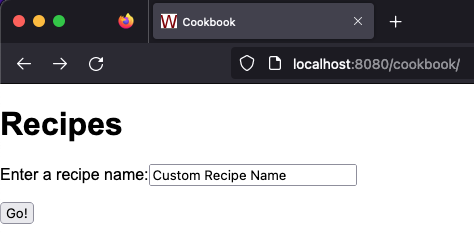
\includegraphics[width=\textwidth]{../img/webdsl-forms-root}
            \caption{\label{fig:webdsl-forms-root-page}Root page}
          \end{subfigure}
          \begin{subfigure}[t]{1\textwidth}
            \capstart
            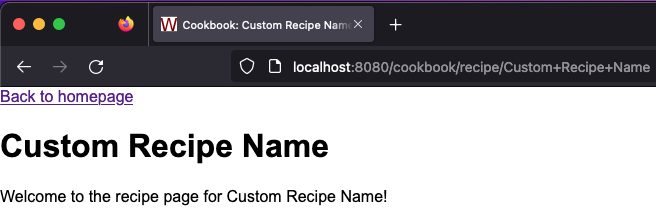
\includegraphics[width=\textwidth]{../img/webdsl-forms-recipe}
            \caption{\label{fig:webdsl-forms-recipe-page}Recipe page}
          \end{subfigure}
        \end{subfigure}
      \caption{\label{fig:webdsl-forms}An example of a WebDSL application that uses a form for navigation.}
      \end{figure}

      \Cref{fig:webdsl-forms} no longer contains a fixed list with links to all possible recipes as in \cref{fig:webdsl-pages-and-templates} but now uses a form with an input and submits an action when the user presses a button. The root page contains a variable declaration as the first line, which defaults to an empty string. In the form later on the page, this variable is passed to an input element. After the input, the form has a button that send a request to the web server to execute the action \texttt{toRecipe} when it is pressed. When this request is sent to the server, the data entered in the input field is linked to variable \texttt{s} by WebDSL, and the action code is able to use this in its body. The return value of an action is the page that should be shown as response. In the example of \cref{fig:webdsl-forms}, the result of executing the action is to show the \texttt{recipe} page with the input that the user has entered in the form.

      WebDSL also sanitizes the input that the user submits using the form. If the user was to submit the form with input \texttt{another/path/}, this input would be sanitized and rendered correctly on the recipe page, instead of navigation to an unknown path.

      Note that WebDSL usually has declare-before-use semantics inside in page, templates or function bodies, but actions can be declared and resolved anywhere in a page or template definition.

    \subsection{\label{subsec:template-overloading}Template Overloading}

      Templates in WebDSL must have a unique combination of name and argument types. This means that, similar to functions in Java, WebDSL supports overloading the same template with different arguments. The built-in \texttt{input} template that is used in previous subsection is an example of this. In \cref{fig:webdsl-forms}, a string argument is passed to the \texttt{input} template which rendered a text field on the resulting web page.

      \Cref{fig:webdsl-template-overloading} shows an example of template overloading. The \texttt{describe} template is defined multiple times for different argument types. The \texttt{input} template is provided by the WebDSL standard library and also defines different input elements for different types.

      \begin{figure}
        \begin{subfigure}[t]{0.45\textwidth}
          \begin{minted}[firstline=1]{\webdsl}
application app
  page root {
    var s : String
    var b : Bool
    var t : Text
    var d : Date

    title { "Input Examples" }

    header { "Input Examples" }

    form {
      par {
        describe(s)
        input(s)
      }
      par {
        describe(b)
        input(b)
      }
      par {
        describe(t)
        input(t)
      }
      par {
        describe(d)
        input(d)
      }
    }
  }

  template describe(s : String) { "String input:" }
  template describe(b : Bool)   { "Bool input:"   }
  template describe(t : Text)   { "Text input:"   }
  template describe(d : Date)   { "Date input:"   }
          \end{minted}
          \caption{\label{fig:webdsl-template-overloading-webdsl}WebDSL code}
        \end{subfigure}
        \begin{subfigure}[t]{0.55\textwidth}
          \capstart
          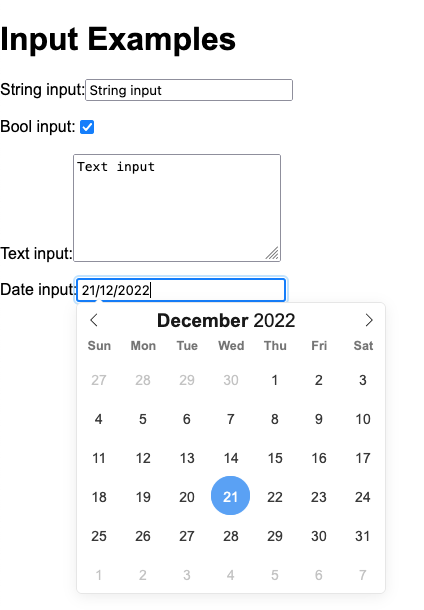
\includegraphics[width=\textwidth]{../img/webdsl-template-overloading}
          \caption{\label{fig:webdsl-template-overloading-page}Resulting page}
        \end{subfigure}
      \caption{\label{fig:webdsl-template-overloading}An example of template overloading in WebDSL with inputs and descriptions.}
      \end{figure}

      In WebDSL, multiple text-based types such as \texttt{String}, \texttt{Text}, \texttt{WikiText} and \texttt{Secret} are all compatible with the base type \texttt{String}. When the arguments are passed to a template, it resolves the most specific template. An example of this is that \texttt{describe(t)} in \cref{fig:webdsl-template-overloading} is compatible with \texttt{String} and \texttt{Text}, but it resolves to the definition with a \texttt{Text} argument.

      When a template call has multiple arguments, it resolves to the template where all arguments are the most specific. If there is one template definition where the first argument is more specific, and another definition where the second argument is more specific, this is incorrect code and the WebDSL development environment shows an error to the developer.

    \subsection{\label{subsec:ajax}Ajax}

      To enable refreshing or replacing parts of a page with new content that is fetched from the server, WebDSL has support for placeholders that can be populated with content using \textit{asynchronous JavaScript and XML} (ajax). Without ajax functionalities, refreshing data on a page would require a full page reload.

      \Cref{fig:webdsl-ajax} shows an example WebDSL application that defines an initially empty placeholder named \texttt{ph}. On the bottom of the page, a clickable link with an inline action is defined. When the action is executed, it will replace the content of the placeholder with the content of the ajax-enabled template \texttt{hello()}. The calling of the action does not incur a full page refresh, but instead fires an asynchronous request that returns the content of the ajax template, after which the placeholder content is replaced using JavaScript.

      \begin{figure}
        \begin{subfigure}[t]{0.45\textwidth}
          \begin{minted}[firstline=1]{\webdsl}
application app
  page root {
    title { "Ajax Example" }

    header { "Ajax Example" }

    par {
      placeholder ph {}
    }

    submitlink action {
      replace(ph, hello());
    } { "Replace" }
  }

  ajax template hello {
    "Hello!"
  }
          \end{minted}
          \caption{\label{fig:webdsl-ajax-webdsl}WebDSL code}
        \end{subfigure}
        \begin{subfigure}[t]{0.55\textwidth}
        \begin{subfigure}[t]{1\textwidth}
          \capstart
          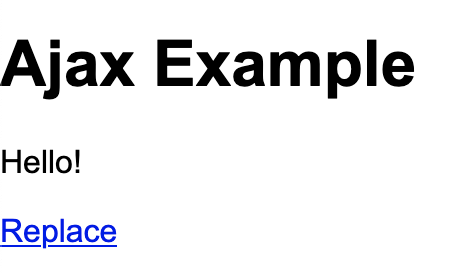
\includegraphics[width=0.75\textwidth]{../img/webdsl-ajax-1}
          \caption{\label{fig:webdsl-ajax-page-1}Resulting page}
        \end{subfigure}
        \begin{subfigure}[t]{1\textwidth}
          \capstart
          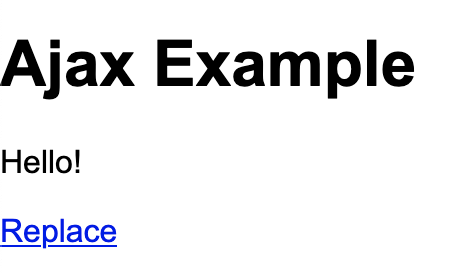
\includegraphics[width=0.75\textwidth]{../img/webdsl-ajax-2}
          \caption{\label{fig:webdsl-ajax-page-2}After clicking the link}
        \end{subfigure}
      \end{subfigure}[t]
      \caption{\label{fig:webdsl-ajax}An example of placeholders and ajax actions in WebDSL.}
      \end{figure}

      WebDSL automatically takes care of the necessary structure to enable this functionality, such as identifiers of DOM elements, JavaScript code to query the server and JavaScript code to replace the correct elements.

      As opposed to regular templates, ajax-enabled template can be requested on the server using a specific endpoint. The exact details of how this endpoint looks is only relevant for generated code of the WebDSL compiler, but WebDSL developers should pay attention to the fact that ajax-enabled content must be projected with proper access control rules (see \cref{sec:access-control}) to prevent exposing sensitive content.

    \subsection{\label{subsec:redefines}Dynamically Scoped Redefines}

      As last part of the user interface section, we give an example of dynamically scoped redefines in WebDSL. WebDSL templates can be redefined (i.e. overridden) inside another template. The redefined content will be shown when the redefined template is used within the template that redefines it. This also holds for calls to the redefined template, nested arbitrarily deep.

      \Cref{fig:webdsl-template-overriding} shows an example of a dynamically scoped redefinition of a template. In the figure, \texttt{templateB} redefines \texttt{templateA}, resulting in the overridden template being rendered when it is called within \texttt{templateB}. To prove that this is scoped, \texttt{templateA} is called before and after \texttt{templateB} and it renders the same (original) text. In the example of \cref{fig:webdsl-template-overriding}, the redefined template is called directly from the template where it is redefined, but it has the same effect when it would be called in nested templates.

      \begin{figure}
        \begin{subfigure}[t]{0.45\textwidth}
          \begin{minted}[firstline=1]{\webdsl}
application app
  page root {
    title { "Override Template" }

    header { "Override Template" }

    templateA
    templateB
    templateA
  }

  template templateA {
    par {
      "I'm Template A!"
    }
  }

  template templateB {
    // override template A
    template templateA {
      par {
        "I'm Template A inside template B!"
      }
    }

    par {
      "I'm Template B!"
    }
    templateA
  }
          \end{minted}
          \caption{\label{fig:webdsl-template-overriding-webdsl}WebDSL code}
        \end{subfigure}
        \begin{subfigure}[t]{0.55\textwidth}
          \capstart
          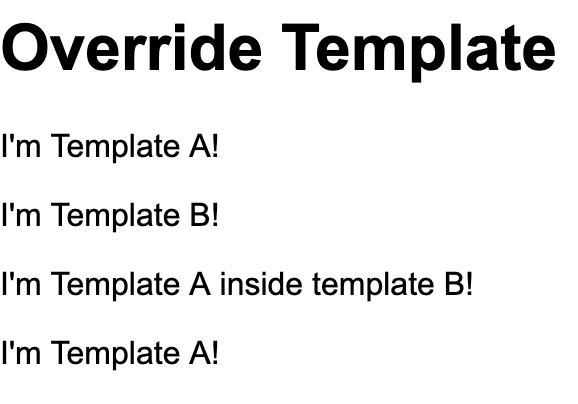
\includegraphics[width=\textwidth]{../img/webdsl-template-overriding}
          \caption{\label{fig:webdsl-template-overriding-page}Resulting page}
        \end{subfigure}
      \caption{\label{fig:webdsl-template-overriding}An example of template overriding in WebDSL.}
      \end{figure}

      Apart from this redefinition of templates inside the context of other templates, WebDSL also has a notion of a one-time global redefinition. This is done using the keyword \texttt{override} on a template in the global scope. The WebDSL standard library contains many definitions that are able to be used by developers, such as an access-denied page, a login template or the input templates that are used in \cref{fig:webdsl-template-overloading}. Using the \texttt{override} keyword, developers are able to customize the style and behavior of these templates.

  \section{\label{sec:data-model}Data Model}

    The data model of a WebDSL application is defined using entities. Entities can have properties and relations with other entities. WebDSL translates the entities to database tables and columns such that any data stored in entities is persisted. The communication with the database is abstracted by WebDSL, allowing WebDSL developers to easily access, manipulate and pass around entity values.

    \Cref{fig:webdsl-data-model-simple} shows an example of an application with stored recipes. A \texttt{Recipe} has two properties: a name and a duration. The application is similar to the earlier representation from \cref{fig:webdsl-pages-and-templates} where a recipe was simply defined by its name, encoded as a String. The representation using entities now defines the \texttt{recipe} page which takes a Recipe as argument, demonstrating how entities are represented in the WebDSL type system.

    \begin{figure}
      \begin{subfigure}[t]{0.45\textwidth}
        \begin{minted}[firstline=1]{\webdsl}
application cookbook

section data model
  entity Recipe {
    name            : String
    minutesRequired : Int
  }

  init {
    var r1 := Recipe {
      name := "Lasagne",
      minutesRequired := 60
    };
    var r2 := Recipe {
      name := "Pancakes",
      minutesRequired := 20
    };
    var r3 := Recipe {
      name := "Tomato Soup",
      minutesRequired := 40
    };
  }

section user interface
  page root {
    title { "Cookbook" }
    header { "Recipes" }
    for (r : Recipe) {
      par {
        navigate recipe(r) { "View recipe for ~r.name" }
      }
    }
  }

  page recipe(r : Recipe) {
    title { "Cookbook: ~r.name" }
    navigate root() { "Back to homepage" }
    header { "~r.name" }
    par {
      "Welcome to the recipe page for ~r.name!"
    }
    par {
      "Minutes required: ~r.minutesRequired"
    }
  }
        \end{minted}
        \caption{\label{fig:webdsl-data-model-simple-webdsl}WebDSL code}
      \end{subfigure}
      \begin{subfigure}[t]{0.55\textwidth}
        \capstart
        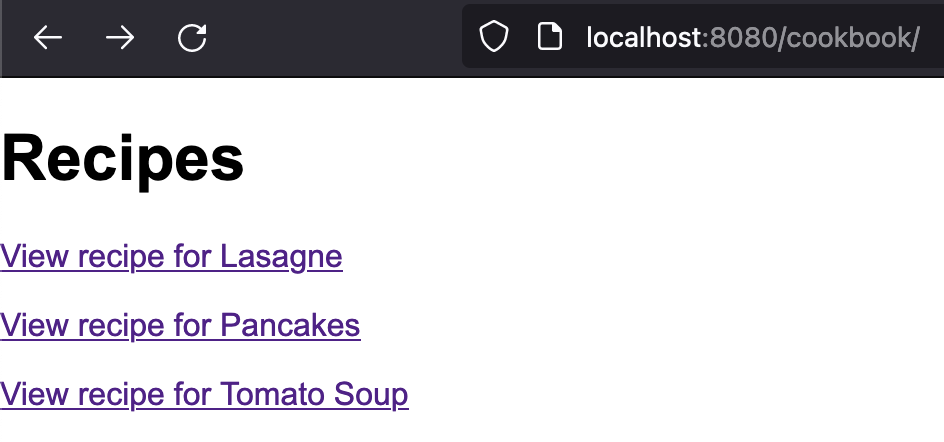
\includegraphics[width=\textwidth]{../img/webdsl-data-model-simple-root}
        \caption{\label{fig:webdsl-data-model-simple-root}Root page}
      \end{subfigure}
      \begin{subfigure}[t]{1\textwidth}
        \capstart
        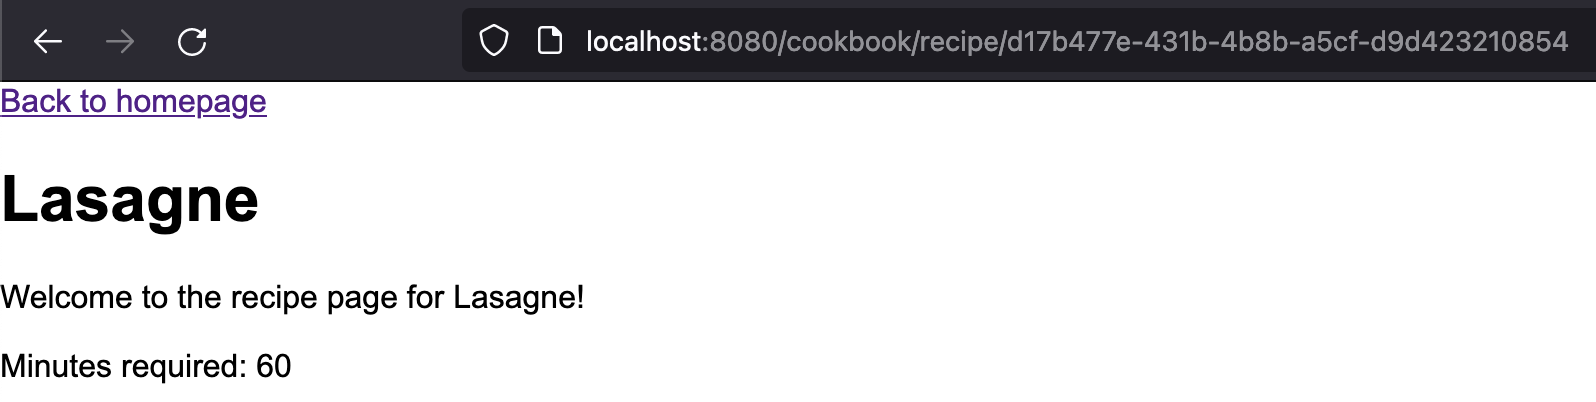
\includegraphics[width=\textwidth]{../img/webdsl-data-model-simple-recipe}
        \caption{\label{fig:webdsl-data-model-simple-recipe}Recipe page}
      \end{subfigure}
    \caption{\label{fig:webdsl-data-model-simple}An example of template overriding in WebDSL.}
    \end{figure}

    The \texttt{init\{\}} block in the global scope of \cref{fig:webdsl-data-model-simple} is executed only once, and often used to seed the database.

    Furthermore, the root page of \cref{fig:webdsl-data-model-simple} uses a for-loop to iterate over all existing instances of an entity; Recipes in our case. It is uncommon to loop over \textit{all} entities, thus WebDSL supports a filter in the for-loop similar to SQL syntax.

    \subsection{\label{subsec:webdsl-inheritance}Entity Inheritance}

      WebDSL allows entity inheritance, meaning that an entity can be a sub-entity of another entity. Similar to subclasses in Java, sub-entities inherit all properties from their parent and are able to define properties of their own.

    \subsection{\label{subsec:webdsl-entity-extension}Entity Extension}

      In the process of developing applications with WebDSL, entities tend to grow in size. For new features in an application, additional properties and functions are added to existing entities. To prevent having a single large entity declaration, WebDSL supports extending existing entities in multiple declarations, similar to partial classes in C\#. Entity extensions are able to use all properties from other extensions and are not self-contained.

      During compilation all entity extensions are merged, resulting in a large entity definition that is represented in the database in a single table.

  \section{\label{sec:access-control}Access Control}

    \begin{figure}
      \begin{minted}[firstline=1]{\webdsl}
application accesscontrol

section data model
  entity User {
    username : String
    password : Secret
    role : String
  }

section user interface
  page root {
    welcome
    secureContent
  }

  template welcome {
    if (loggedIn) { "Hello ~principal.username" }
    else          { "Hello unknown user" }
  }

  template secureContent {
    "This is only visible while logged in "
    "due to access control"

    submit a() { "Click!" }
    action a() {
      adminOnlyFunction();
    }
  }

access control rules
  principal is User 
    with credentials username, password

  // pages are hidden by default
  rule page root() { true }

  // templates are visible by default
  rule template secureContent() {
    loggedIn
    rule action a() {
      principal.role == "admin"
    }
  }
      \end{minted}
      \caption{\label{fig:webdsl-access-control}Access control in WebDSL}
    \end{figure}

    Almost all web applications use a form of access control. Examples of access control are using a log-in system, allowing users to only edit content of which they are the author, or the assigning of roles to groups of users in a large organization.

    WebDSL recognizes the need for secure access control and provides a functionality where an entity is appointed as the user entity with some credentials. A policy can be assigned to all pages, templates and actions in WebDSL in a declarative way and separated from the implementation. Using the built-in access control functionality, WebDSL developers do not have to deal with communication and security details such as cookies and hashing.

    \Cref{fig:webdsl-access-control} shows an example of a WebDSL application with access control rules. The entity \texttt{User} is declared as the entity for access control using its properties \texttt{username} and \texttt{password}. Declaring the principal causes some properties to be exposed for handling access control such as \texttt{loggedIn} of boolean type and \texttt{principal} of type \texttt{User}. Multiple rules are declared for the root page, the templates and the action within a template.

    In addition to these individual rules, WebDSL allows reuse of access control rules through predicates that can be called from individual rules or pointcuts to which multiple pages and templates are assigned. Furthermore, the matching of access control rules may contain wildcards in the name or arguments to prevent specifying the same rule multiple times for an overloaded template.

    WebDSL infers the visibility of pages and elements on a page from the access control rules. For example, in case a page features a link to another page and the user does not have access to the other page according to the access control rules, the link will not be shown. If a user explicitly browses to the other page, it will show an access denied page that is provided by WebDSL by default but is customizable.

  \section{\label{sec:functions}Functions}

  \begin{figure}
    \begin{minted}[firstline=1]{\webdsl}
application cookbook
entity Recipe {
  name : String
  minutesRequired : Int
  author : User

  // extend generated setter
  extend function setAuthor(u : User) {
    log("Set the author to ~u.username");
  }
}

entity User {
  username : String
  password : Secret

  function appendUsername(s : String) {
    this.username := this.username + s;
  }
}

// sub-entity Admin of with parent User
entity Admin : User {
  // override behaviour
  function appendUsername(s : String) {
    this.username := this.username + "admin" + s;
  }
}

function globalFunction() : Int {
  var x := 40;
  return x + 2;
}

template outputFortyTwo {
  var i := globalFunction();

  "~i"
}
    \end{minted}
    \caption{\label{fig:webdsl-functions}Functions in WebDSL}
  \end{figure}

    Most WebDSL constructs in previous sections are specified declaratively. However, WebDSL also supports imperative code using functions. Similar to Java functions, WebDSL functions can be scoped globally, or belong to a certain entity. These functions are able to take arguments and return a value of a certain type. Additionally, WebDSL generates many functions based on the declared entities and properties, some of which serve as hook and can be extended.

    \Cref{fig:webdsl-functions} showcases some function behavior of WebDSL. It demonstrates extending a generated setter-function of the entity \texttt{Recipe}. The \texttt{setAuthor} function, including its extension, will be called when the author of a recipe is changed. Next, the entity \texttt{User} has an entity function \texttt{appendUsername}, of which the behavior is overridden in the \texttt{Admin} sub-entity. Lastly, a global function is defined, and a template demonstrates how the template body and function code can interact.
  
  \section{\label{sec:advanced-webdsl-features}Advanced WebDSL Features}

    In the previous sections we listed the fundamental concepts of WebDSL that are necessary to create everyday systems. However, WebDSL enjoys more features which give the developer even more customization options.

    \paragraph{Native Java Code} WebDSL compiles to Java and abstracts over necessary boilerplate code to make a functioning web application with Java. However, these abstractions prevent some concepts from being expressible in WebDSL code. For this reason, it is possible to create Java files in a WebDSL project and provide an interface in the WebDSL code such that the definitions in the Java code are able to be typed and usable in WebDSL code. Such a definition of an interface in WebDSL is called a Native Java Class.

    \paragraph{Built-in Type Extension} In \cref{subsec:webdsl-entity-extension} we described the possibility of extending entities in WebDSL across multiple files. This same feature is available for extending built-in types such as \texttt{String}, \texttt{Bool} and the root of the type hierarchy \texttt{Object}. The built-in types translate to their respective Java types, and with type extension it is possible to expose additional functions of the Java type to the WebDSL code, that are not exposed by default.

    \paragraph{Search} Van Chastelet (\citeyear{VanChastelet2013}) extended WebDSL with a search-feature based on Lucene\footnote{\url{https://lucene.apache.org/}}. For applications with a large quantity of data such as researchr.org\footnote{\url{https://researchr.org/}} it is useful to make the data discoverable through search. As the amount data increases, implementing a search feature through querying the database becomes infeasible. The WebDSL search features allows entity properties to be annotated with a \texttt{searchable} annotation, declaring that they should be indexed. Through these annotations and advanced search mappings, it is possible to for example use fuzzy search on enormous amounts of data and search on multiple entity properties at the same time.

    \paragraph{Routing} By default, WebDSL translates pages to URLs as follows.
    $$
    https://<domainname>/<pagename>/<arg\_1>/<arg\_2>/.../<arg\_n> 
    $$
    For most cases this suffices, but it is possible to declare a \texttt{routing} block in WebDSL where the developer is able to intercept the requested URL, extract the page name and arguments, apply logic based on those and return the desired page in WebDSL.

  \section{\label{sec:current-implementation}Current Implementation of WebDSL}

    In the paper where Visser first introduced WebDSL (\citeyear{Visser2007}), it is presented as a large case study in domain-specific language engineering. Visser describes the implementation of the language with its syntax definition and code generation by term transformation using the Stratego/XT toolset.

    The Stratego/XT toolset \autocite{BravenboerKVV08} offers a set of features for syntax definition (with SDF2), program transformation (with Stratego)  and various tools such as parser and pretty-printer generators. Stratego/XT is the predecessor of the Spoofax language workbench \autocite{KatsV10}. Spoofax offers an IDE for language engineers using an Eclipse plugin and features more meta-languages, each specialized for different components of a language definition.
    
    The core of the current WebDSL implementation is still the same, 15 years later. While the language has matured and is extended in many useful ways, the syntax is still defined in SDF2 and the rest of the compilation chain is implemented in Stratego, using the Stratego/XT toolset which is not actively developed anymore.
    
    An application in WebDSL is compiled to a Java program, and a persisted data model through the use of the Hibernate Query Language (HQL) in the generated Java code. Before the correct target code can be generated, the WebDSL code has to pass the compilation chain that consists of components such as the parser, desugaring, type checking. In the rest of this section we discuss the implementation of the WebDSL static analysis in Stratego. In the next chapter (\cref{chap:sdf3}), we describe the parser generated from the WebDSL SDF2 definition.

    \subsection{WebDSL in Stratego}

      Apart from the syntax definition, every component of the WebDSL compiler is implemented in Stratego. For the scope of this thesis, we will focus on the implementation of the WebDSL static analysis in Stratego and we will not discuss the implementation of code generation.

      Stratego \autocite{BravenboerDOV06,VisserBT98} is a transformation language based on term rewriting. Stratego enables the definition of strategies that traverse an abstract syntax tree (AST) and applies rewrite rules. These rewrite rules may be conditional and are of the form $r : t_1 -> t_2\;\texttt{where}\;c$ with r being the name, $t_1$ and $t_2$ are terms and $c$ is the condition. For a complete overview of the capabilities of Stratego, we refer to its documentation\footnote{\url{https://www.spoofax.dev/references/stratego/}}.

      The Stratego code for WebDSL consists of many Stratego rules that match an AST term with some conditions in the where clause that define the analysis. The static analysis is done through returning the same term as matched, but storing errors or warnings in the process. The rule that aggregates the individual rules is called \texttt{constraint-error} and this is applied in a bottom-up fashion. The bottom-up traversal strategy means that the rule will first be applied to subterms, and then to the term itself. The \texttt{constraint-error} rule is composed of many rules for specific WebDSL features. The implementation and usage of \texttt{constraint-error} is shown in \cref{fig:webdsl-stratego-constraint-error}.

      \begin{figure}
        \begin{minted}[firstline=2]{\stratego}
module org/webdsl/dsl/languages/composition
  strategies
    constraint-error-all = bottomup(try(constraint-error))

    constraint-error = constraint-error-ac
    constraint-error = constraint-error-data
    constraint-error = constraint-error-action
    constraint-error = constraint-error-ui
    constraint-error = constraint-error-search
    // ...
        \end{minted}
        \caption{\label{fig:webdsl-stratego-constraint-error}Definition of the WebDSL type checking framework in Stratego. Some rules are ommitted for brevity.}
      \end{figure}

      Stratego aggregates all definitions of the same rule from multiple files and combines them into one rule. The WebDSL implementation in Stratego relies on this feature by defining multiple rules with the same name, but matching on different elements with different conditions. An example of a WebDSL static analysis rule in Stratego is shown in \cref{fig:webdsl-stratego-typecheck}.

      \begin{figure}
        \begin{minted}[firstline=2]{\stratego}
module org/webdsl/dsl/languages/composition
  rules
    constraint-error-ac =
      ?AccessControlPrincipal(_,_)
    ; where(principals := <bagof-PrincipalDecl; uniq; length>)
    ; where(<gt> (principals, 1))
    ; add-error(|["Only one access control principal can be defined."])

    add-error(|msgs) =
      rules(
        FoundErrors := <inc> <FoundErrors <+ !0>
      )
      ; try(AddError(|msgs))

    AddError(|msgs): node -> node
      where rules(
        AllErrors :+= (node, <error-to-string> msgs)
      )
        \end{minted}
        \caption{\label{fig:webdsl-stratego-typecheck}Definition of Stratego rule that shows an error message when two principals are declared in the access control rules of WebDSL.}
      \end{figure}

      The \texttt{add-error} and \texttt{AddError} in \cref{fig:webdsl-stratego-typecheck} utilize dynamic rules in Stratego using the \texttt{rules(...)} block. Similar to (normal) rules in Stratego, a dynamic rule matches a term, returns a term and is able to have conditions. When dynamic rules are added during the execution of a Stratego program, it is added to the possible set of rules that can be applied. In the case of the WebDSL implementation, dynamic rules are (ab)used to store data, possibly limited to a certain scope, about the WebDSL program that is being compiled.

      In the implementation, scoped dynamic rules are heavily utilized to store the internal state of the compiler. We argue that the extensive use of (scoped) dynamic rules obstructs the elegance, readability and maintainability of the WebDSL implementation in Stratego, because the effect of the dynamic rules are hard to predict before running the compiler without extensive experience with the codebase.

  \section{\label{sec:modernization}Modernization Goal}

    As discussed in the previous section, WebDSL is implemented in the Stratego/XT toolset which is not actively maintained anymore. Spoofax is the successor of the deprecated Stratego/XT toolset and features an extensive meta-languages, each specialized for defining different components of a language in a declarative way.

    SDF3 \autocite{VollebregtKV12,AmorimV20} is the meta-language in Spoofax for syntax definition in a declarative way. From an SDF3 grammar, Spoofax generates a parser, a pretty-printer and syntactic code completions. Statix \autocite{VanAntwerpen2018} is a constraint-based declarative language for the specification of type systems in Spoofax, using the concept of scope graphs \autocite{Neron2015} to model programs.

    In this thesis we modernize the WebDSL front-end by defining the WebDSL grammar in SDF3 without post-parse filters and the WebDSL static semantics in Statix. Using this process and result, we hope to gain insight into the completeness, expressiveness and elegance of Statix and SDF3 when they are used to implement a real world language by answering the following research questions.

    \begin{itemize}
      \item \textbf{RQ1} Is it possible to define the WebDSL syntax in SDF3, without the use of post-parse filters?
      \item \textbf{RQ2} How does the run time efficiency of the parser generated from WebDSL in SDF3 compare to the current WebDSL parser generated from SDF2?
      \item \textbf{RQ3} How does the maintainability of WebDSL in SDF3 compare to the WebDSL syntax definition in SDF2?
      \item \textbf{RQ4} Is a Statix implementation of the WebDSL static semantics able to catch the same errors and warnings as the current implementation in Stratego?
      \item \textbf{RQ5} How does the run time efficiency of the WebDSL static semantics in Statix compare to the current WebDSL implementation?
      \item \textbf{RQ6} How does the maintainability of the WebDSL static semantics in Statix compare to the current implementation?
    \end{itemize}
